% pe_basics.tex -- The processing element (PE), visually, for beginners (Lab 3 companion)
% Build:  tectonic pe_basics.tex      (or: pdflatex pe_basics.tex, run twice)
\documentclass[aspectratio=169,11pt]{beamer}

\usepackage{tikz}
\usetikzlibrary{arrows.meta,positioning,shapes.geometric,calc,fit}
\usepackage{booktabs}
\usepackage{listings}
\usepackage{amssymb}
\usepackage{pifont}

% ---------------- look (same palette as the other decks) ----------------
\definecolor{pcb}{HTML}{0B2E33}
\definecolor{pcbmid}{HTML}{1F5C61}
\definecolor{tint}{HTML}{E6F0EF}
\definecolor{copper}{HTML}{B5651D}
\definecolor{coppert}{HTML}{F6E8DC}
\definecolor{ink}{HTML}{1F2A2E}
\definecolor{muted}{HTML}{5B6B70}
\definecolor{codebg}{HTML}{F4F7F7}
\definecolor{good}{HTML}{2E7D32}
\definecolor{bad}{HTML}{B3261E}

\usetheme{default}
\setbeamercolor{background canvas}{bg=white}
\setbeamercolor{frametitle}{fg=pcb}
\setbeamercolor{normal text}{fg=ink}
\setbeamercolor{structure}{fg=pcbmid}
\setbeamerfont{frametitle}{series=\bfseries,size=\Large}
\setbeamertemplate{navigation symbols}{}
\setbeamertemplate{itemize item}{\color{copper}$\blacktriangleright$}
\setbeamertemplate{footline}{\hfill\color{muted}\scriptsize\insertframenumber\hspace{1.2em}\vspace{0.6em}}

\newcommand{\sig}[1]{\texttt{#1}}

\lstset{basicstyle=\ttfamily\fontsize{7.2}{8.6}\selectfont, backgroundcolor=\color{codebg},
  frame=single, rulecolor=\color{pcbmid}, keywordstyle=\color{pcbmid}\bfseries,
  commentstyle=\color{muted}\itshape, columns=fullflexible, keepspaces=true,
  morekeywords={logic,always_ff,signed,parameter,int,module,endmodule,input,output,assign,posedge,begin,end,if,else},
  xleftmargin=2pt, xrightmargin=2pt}

\tikzset{
  blk/.style  ={draw=pcbmid, fill=tint, rounded corners=3pt, thick, align=center,
                font=\footnotesize, inner sep=4pt},
  hot/.style  ={draw=copper, fill=coppert, rounded corners=3pt, thick, align=center,
                font=\footnotesize, inner sep=4pt},
  reg/.style  ={draw=pcb, fill=white, thick, align=center, font=\footnotesize,
                minimum width=16mm, minimum height=8mm},
  wire/.style ={-{Stealth[length=2mm]}, thick, copper},
  wireb/.style={-{Stealth[length=2mm]}, thick, pcbmid},
  lbl/.style  ={font=\scriptsize\ttfamily, fill=white, inner sep=1pt},
  w/.style    ={font=\scriptsize, text=muted, fill=white, inner sep=1pt},
}

% timing-diagram helpers (x in cycles, 1 cycle = 1.45 cm)
\newcommand{\bus}[4]{% x0 x1 y text
  \draw[pcbmid] (#1*1.45+0.08,#3) -- (#1*1.45+0.16,#3+0.22) -- (#2*1.45-0.08,#3+0.22) -- (#2*1.45,#3)
                -- (#2*1.45-0.08,#3-0.22) -- (#1*1.45+0.16,#3-0.22) -- cycle;
  \node[font=\tiny\ttfamily] at ({(#1+#2)*0.725+0.04},#3) {#4};}

\title{\textcolor{pcb}{The Processing Element (PE)}}
\subtitle{From the idea to the RTL, one picture at a time}
\author{Lab 3 companion \textperiodcentered{} systolic-array project}
\date{}

\begin{document}

% =====================================================================
\begin{frame}
  \titlepage
  \centering\color{muted}\small
  Read this before writing \sig{labs/my\_rtl/pe.sv}. The code itself is on the last slides ---
  look at it only after your own version passes \sig{tb/test\_pe.py}.
\end{frame}

% =====================================================================
\begin{frame}{1.\ Where the PE sits: one small box, copied 16 times}
  \begin{columns}[T]
    \column{0.5\textwidth}
    \centering
    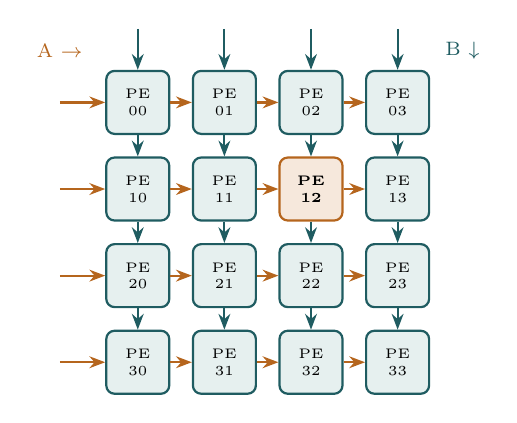
\begin{tikzpicture}[x=11mm,y=11mm]
      \foreach \i in {0,...,3} \foreach \j in {0,...,3} {
        \ifnum\i=1 \ifnum\j=2
          \node[hot, minimum size=8mm, inner sep=0pt, font=\tiny\bfseries] (p\i\j) at (\j,-\i) {PE\\\i\j};
        \else
          \node[blk, minimum size=8mm, inner sep=0pt, font=\tiny] (p\i\j) at (\j,-\i) {PE\\\i\j};
        \fi
        \else
          \node[blk, minimum size=8mm, inner sep=0pt, font=\tiny] (p\i\j) at (\j,-\i) {PE\\\i\j};
        \fi
      }
      \foreach \i in {0,...,3} \foreach \j/\jn in {0/1,1/2,2/3} \draw[wire] (p\i\j) -- (p\i\jn);
      \foreach \j in {0,...,3} \foreach \i/\inn in {0/1,1/2,2/3} \draw[wireb] (p\i\j) -- (p\inn\j);
      \foreach \i in {0,...,3} \draw[wire] (-0.9,-\i) -- (p\i0);
      \foreach \j in {0,...,3} \draw[wireb] (\j,0.85) -- (p0\j);
      \node[font=\scriptsize, text=copper] at (-0.9,0.6) {A $\rightarrow$};
      \node[font=\scriptsize, text=pcbmid] at (3.75,0.6) {B $\downarrow$};
    \end{tikzpicture}
    \column{0.47\textwidth}\small
    \begin{itemize}
      \item The 4$\times$4 array is \textbf{16 identical PEs}.
      \item \textcolor{copper}{\textbf{A}} values move \textbf{right}, \textcolor{pcbmid}{\textbf{B}} values
            move \textbf{down}, one step per clock.
      \item The highlighted \textbf{PE(1,2)} builds one answer: \textbf{C[1][2]}.
      \item Design \textbf{one} PE correctly and the whole array works. A bug in it breaks \textbf{every} result.
    \end{itemize}
  \end{columns}
\end{frame}

% =====================================================================
\begin{frame}{2.\ What one PE does every clock: three jobs}
  \centering
  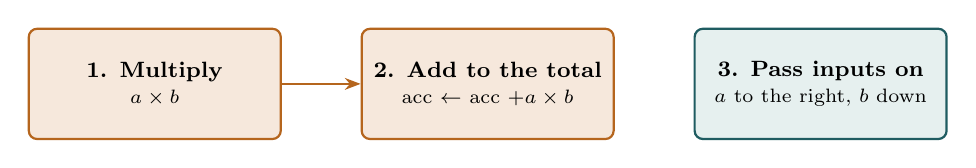
\begin{tikzpicture}[node distance=6mm and 10mm]
    \node[hot, minimum width=32mm, minimum height=14mm] (j1) {\textbf{1. Multiply}\\\scriptsize $a \times b$};
    \node[hot, right=of j1, minimum width=32mm, minimum height=14mm] (j2) {\textbf{2. Add to the total}\\\scriptsize acc $\leftarrow$ acc $+ a\times b$};
    \node[blk, right=of j2, minimum width=32mm, minimum height=14mm] (j3) {\textbf{3. Pass inputs on}\\\scriptsize $a$ to the right, $b$ down};
    \draw[wire] (j1) -- (j2);
  \end{tikzpicture}
  \vspace{5mm}

  \raggedright\small
  \begin{itemize}
    \item Jobs 1 and 2 together are a \textbf{MAC} (multiply-accumulate). After K clocks, \sig{acc} holds
          one dot product: $\sum_k A[i][k]\cdot B[k][j]$ = \textbf{C[i][j]}.
    \item Job 3 is what makes it \emph{systolic}: the same $a$ and $b$ are reused by the next PEs.
    \item Two control inputs decide \emph{whether} to work:
          \sig{en} (do a MAC this clock) and \sig{clear} (start a new job: total back to 0).
  \end{itemize}
\end{frame}

% =====================================================================
\begin{frame}{3.\ Inside the PE: the hardware, with bit widths}
  \centering
  \resizebox{0.92\textwidth}{!}{%
  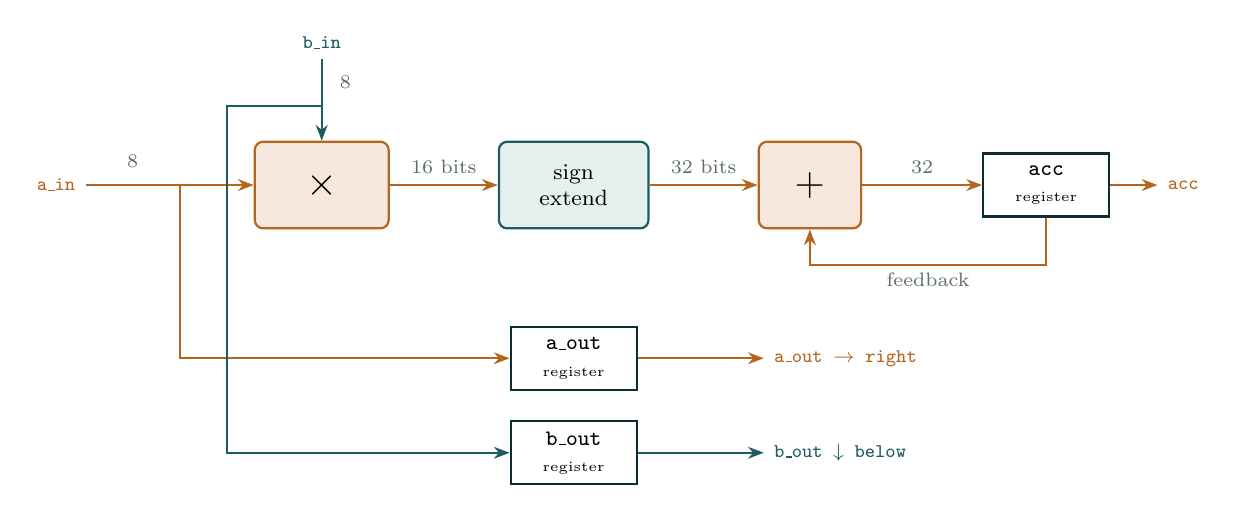
\begin{tikzpicture}[x=1mm,y=1mm]
    \node[hot, minimum width=17mm, minimum height=11mm] (mul) at (30,20) {\Large$\times$};
    \node[blk, minimum width=19mm, minimum height=11mm] (ext) at (62,20) {sign\\extend};
    \node[hot, minimum width=13mm, minimum height=11mm] (add) at (92,20) {\Large$+$};
    \node[reg] (acc) at (122,20) {\sig{acc}\\\tiny register};
    \node[reg] (ar) at (62,-2) {\sig{a\_out}\\\tiny register};
    \node[reg] (br) at (62,-14) {\sig{b\_out}\\\tiny register};
    % inputs
    \draw[wire] (0,20) node[left,font=\scriptsize\ttfamily]{a\_in} -- (mul.west);
    \draw[wireb] (30,36) node[above,font=\scriptsize\ttfamily]{b\_in} -- (mul.north);
    \draw[wire] (mul) -- node[w,above=1mm]{16 bits} (ext);
    \draw[wire] (ext) -- node[w,above=1mm]{32 bits} (add);
    \draw[wire] (add) -- node[w,above=1mm]{32} (acc);
    \draw[wire] (acc.east) -- ++(6,0) node[right,font=\scriptsize\ttfamily]{acc};
    \draw[wire] (acc.south) -- ++(0,-6) -| (add.south);
    \node[w] at (107,8) {feedback};
    % pass-through
    \draw[wire] (12,20) |- (ar.west);
    \draw[wireb] (30,30) -| (18,-14) -- (br.west);
    \draw[wire] (ar.east) -- ++(16,0) node[right,font=\scriptsize\ttfamily]{a\_out $\rightarrow$ right};
    \draw[wireb] (br.east) -- ++(16,0) node[right,font=\scriptsize\ttfamily]{b\_out $\downarrow$ below};
    \node[w] at (6,23) {8};
    \node[w] at (33,33) {8};
  \end{tikzpicture}}
  \vspace{1mm}

  \raggedright\small
  Three \textbf{registers} (boxes with a white fill) update on the rising clock edge; the
  multiplier, sign-extend and adder are \textbf{combinational} (no memory).
  Registers: 32 + 8 + 8 = \textbf{48 flip-flops}.
\end{frame}

% =====================================================================
\begin{frame}{4.\ The rules on every rising clock edge}
  \begin{columns}[T]
    \column{0.55\textwidth}
    \centering
    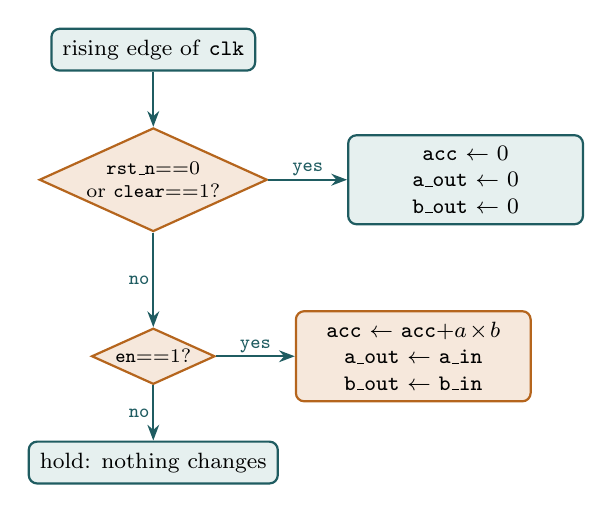
\begin{tikzpicture}[node distance=7mm and 10mm]
      \node[blk] (edge) {rising edge of \sig{clk}};
      \node[diamond, draw=copper, fill=coppert, thick, aspect=2.2, inner sep=1pt, font=\scriptsize,
            align=center, below=of edge] (q1) {\sig{rst\_n}==0\\or \sig{clear}==1?};
      \node[blk, right=of q1, text width=27mm] (zero) {\sig{acc} $\leftarrow$ 0\\\sig{a\_out} $\leftarrow$ 0\\\sig{b\_out} $\leftarrow$ 0};
      \node[diamond, draw=copper, fill=coppert, thick, aspect=2.2, inner sep=1pt, font=\scriptsize,
            below=12mm of q1] (q2) {\sig{en}==1?};
      \node[hot, right=of q2, text width=27mm] (mac) {\sig{acc} $\leftarrow$ \sig{acc}+$a\!\times\!b$\\\sig{a\_out} $\leftarrow$ \sig{a\_in}\\\sig{b\_out} $\leftarrow$ \sig{b\_in}};
      \node[blk, below=7mm of q2] (hold) {hold: nothing changes};
      \draw[wireb] (edge) -- (q1);
      \draw[wireb] (q1) -- node[lbl,above]{yes} (zero);
      \draw[wireb] (q1) -- node[lbl,left]{no} (q2);
      \draw[wireb] (q2) -- node[lbl,above]{yes} (mac);
      \draw[wireb] (q2) -- node[lbl,left]{no} (hold);
    \end{tikzpicture}
    \column{0.42\textwidth}\small
    \begin{itemize}
      \item \textbf{Order matters:} reset/clear is checked \textbf{first}, so \sig{clear} wins
            even when \sig{en} is 1.
      \item \sig{rst\_n} is \textbf{active low}: 0 means reset.
      \item \textbf{Synchronous:} nothing happens between clock edges; the check runs only at the edge.
      \item ``Hold'' needs \textbf{no code}: a register keeps its value when you don't assign it.
    \end{itemize}
  \end{columns}
\end{frame}

% =====================================================================
\begin{frame}{5.\ Why these bit widths}
  \centering
  \resizebox{0.95\textwidth}{!}{%
  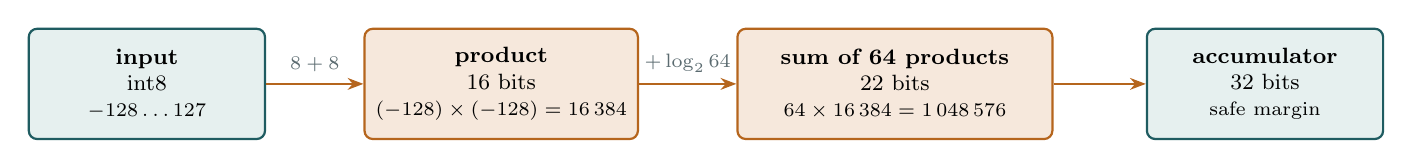
\begin{tikzpicture}[x=1mm,y=1mm]
    \node[blk, minimum width=30mm, minimum height=14mm] (a) at (0,0) {\textbf{input}\\int8\\\scriptsize $-128 \ldots 127$};
    \node[hot, minimum width=34mm, minimum height=14mm] (p) at (45,0) {\textbf{product}\\16 bits\\\scriptsize $(-128)\times(-128) = 16\,384$};
    \node[hot, minimum width=40mm, minimum height=14mm] (s) at (95,0) {\textbf{sum of 64 products}\\22 bits\\\scriptsize $64 \times 16\,384 = 1\,048\,576$};
    \node[blk, minimum width=30mm, minimum height=14mm] (acc) at (142,0) {\textbf{accumulator}\\32 bits\\\scriptsize safe margin};
    \draw[wire] (a) -- node[w,above=1mm]{$8+8$} (p);
    \draw[wire] (p) -- node[w,above=1mm]{$+\log_2 64$} (s);
    \draw[wire] (s) -- (acc);
  \end{tikzpicture}}
  \vspace{5mm}

  \raggedright\small
  \begin{itemize}
    \item \textbf{Multiplying} two $n$-bit numbers needs $2n$ bits.
    \item \textbf{Adding} $K$ numbers needs $\log_2 K$ more bits: 64 products $\rightarrow$ 6 more bits.
    \item 32 bits is safe for any $K$ up to $131\,071$ ($2^{17}-1$); our $K$ is at most 255. Too few bits $\rightarrow$
          the total silently wraps around to a wrong value.
  \end{itemize}
\end{frame}

% =====================================================================
\begin{frame}{6.\ Why \sig{signed} matters}
  \begin{columns}[T]
    \column{0.48\textwidth}
    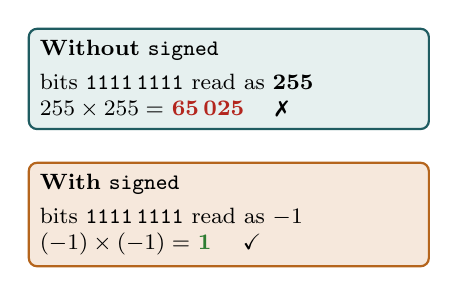
\begin{tikzpicture}[node distance=4mm]
      \node[blk, text width=48mm, align=left] (u) {\textbf{Without \sig{signed}}\\[1mm]
        bits \sig{1111\,1111} read as \textbf{255}\\
        $255 \times 255 = $ \textcolor{bad}{\textbf{65\,025}} \quad \ding{55}};
      \node[hot, text width=48mm, align=left, below=of u] (s) {\textbf{With \sig{signed}}\\[1mm]
        bits \sig{1111\,1111} read as \textbf{$-1$}\\
        $(-1) \times (-1) = $ \textcolor{good}{\textbf{1}} \quad \checkmark};
    \end{tikzpicture}
    \column{0.49\textwidth}\small
    \begin{itemize}
      \item The same 8 bits mean two different numbers; \sig{signed} tells the tools which one.
      \item Declare \sig{a\_in}, \sig{b\_in}, the product and \sig{acc} all \sig{signed}. One
            unsigned operand makes the whole expression unsigned.
      \item \textbf{Trap:} $(-128)\times(-128)$ gives 16\,384 \emph{both} ways ($128 \times 128$ too).
            The test also checks $(-128)\times 127$: $-16\,256$ signed, but $16\,256$ unsigned.
      \item \textbf{Sign extension} copies the top bit when widening 16 $\to$ 32 bits:
            $-5$ = \sig{FFFB} becomes \sig{FFFFFFFB}, not \sig{0000FFFB}.
    \end{itemize}
  \end{columns}
\end{frame}

% =====================================================================
\begin{frame}{7.\ One example, clock by clock}
  \centering
  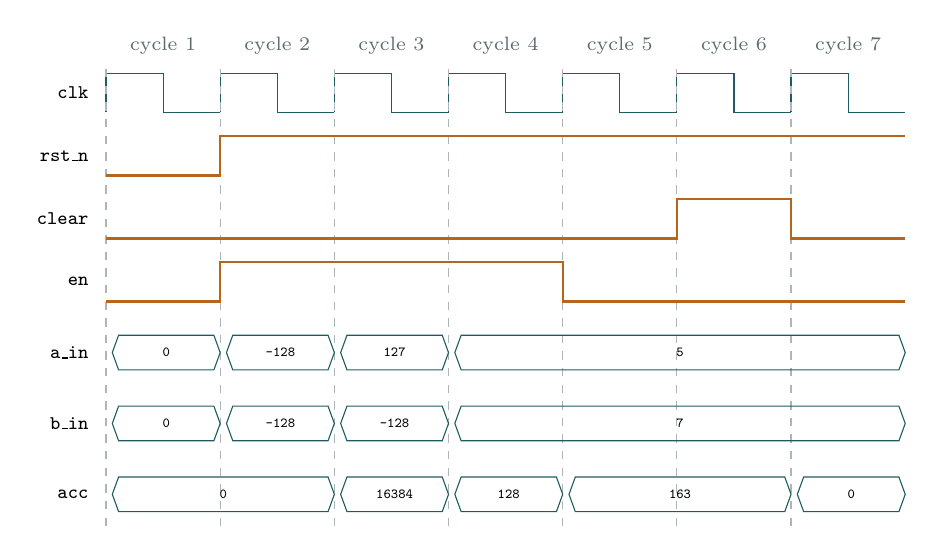
\begin{tikzpicture}[font=\scriptsize]
    \foreach \y/\t in {6/clk, 5.2/rst\_n, 4.4/clear, 3.6/en, 2.7/a\_in, 1.8/b\_in, 0.9/acc}
      \node[anchor=east, font=\scriptsize\ttfamily] at (-0.1,\y) {\t};
    % clock: rising edge at the start of every cycle
    \foreach \c in {0,...,6} {
      \draw[pcbmid] (\c*1.45,5.75) -- (\c*1.45,6.25) -- (\c*1.45+0.725,6.25) -- (\c*1.45+0.725,5.75) -- (\c*1.45+1.45,5.75);
      \draw[muted!50, dashed] (\c*1.45,0.5) -- (\c*1.45,6.35);
    }
    % single-bit signals
    \draw[copper, thick] (0,4.95) -- (1.45,4.95) -- (1.45,5.45) -- (7*1.45,5.45);            % rst_n
    \draw[copper, thick] (0,4.15) -- (5*1.45,4.15) -- (5*1.45,4.65) -- (6*1.45,4.65) -- (6*1.45,4.15) -- (7*1.45,4.15); % clear
    \draw[copper, thick] (0,3.35) -- (1.45,3.35) -- (1.45,3.85) -- (4*1.45,3.85) -- (4*1.45,3.35) -- (7*1.45,3.35);     % en
    % buses
    \bus{0}{1}{2.7}{0} \bus{1}{2}{2.7}{-128} \bus{2}{3}{2.7}{127} \bus{3}{7}{2.7}{5}
    \bus{0}{1}{1.8}{0} \bus{1}{2}{1.8}{-128} \bus{2}{3}{1.8}{-128} \bus{3}{7}{1.8}{7}
    \bus{0}{2}{0.9}{0} \bus{2}{3}{0.9}{16384} \bus{3}{4}{0.9}{128} \bus{4}{6}{0.9}{163} \bus{6}{7}{0.9}{0}
    % cycle numbers
    \foreach \c in {1,...,7} \node[text=muted] at (\c*1.45-0.725,6.6) {cycle \c};
  \end{tikzpicture}
  \vspace{1mm}

  \raggedright\footnotesize
  Inputs are set \textbf{during} a cycle; \sig{acc} changes \textbf{at the next rising edge}.
  Cycle 2's inputs give 16\,384 in cycle 3; then $16\,384 - 16\,256 = 128$; then $128 + 35 = 163$.
  \sig{en} = 0 in cycle 5 holds 163; \sig{clear} in cycle 6 makes it 0.
\end{frame}

% =====================================================================
\begin{frame}[fragile]{8.\ From the picture to the code}
  \begin{columns}[T]
    \column{0.42\textwidth}
    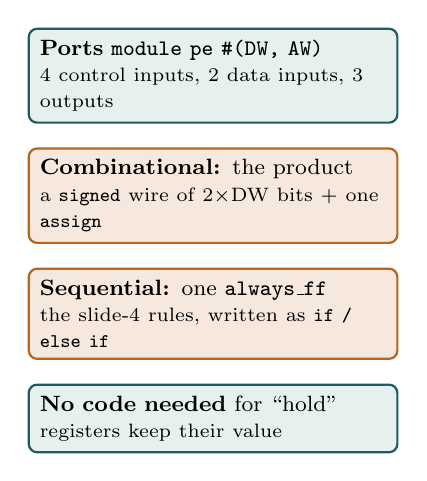
\begin{tikzpicture}[node distance=3mm]
      \node[blk, text width=44mm, align=left] (p) {\textbf{Ports} \sig{module pe \#(DW, AW)}\\\scriptsize 4 control inputs, 2 data inputs, 3 outputs};
      \node[hot, text width=44mm, align=left, below=of p] (m) {\textbf{Combinational:} the product\\\scriptsize a \sig{signed} wire of 2$\times$DW bits + one \sig{assign}};
      \node[hot, text width=44mm, align=left, below=of m] (r) {\textbf{Sequential:} one \sig{always\_ff}\\\scriptsize the slide-4 rules, written as \sig{if / else if}};
      \node[blk, text width=44mm, align=left, below=of r] (n) {\textbf{No code needed} for ``hold''\\\scriptsize registers keep their value};
    \end{tikzpicture}
    \column{0.55\textwidth}
\begin{lstlisting}
module pe #(parameter int DW = 8,
            parameter int AW = 32) (
  input  logic clk, rst_n, clear, en,
  input  logic signed [DW-1:0] a_in, b_in,
  output logic signed [DW-1:0] a_out, b_out,
  output logic signed [AW-1:0] acc
);
  // product: which width? which keyword?
  // assign ... ;

  always_ff @(posedge clk) begin
    if ( /* reset or clear */ ) begin
      // three registers to zero
    end else if ( /* en */ ) begin
      // acc grows by the sign-extended product
      // a_out and b_out copy the inputs
    end
  end
endmodule
\end{lstlisting}
    \footnotesize This is the shape to fill in for Lab 3, Part C. Use \sig{<=} for every register.
  \end{columns}
\end{frame}

% =====================================================================
\begin{frame}[fragile]{9.\ How the tools check your PE}
  \centering
  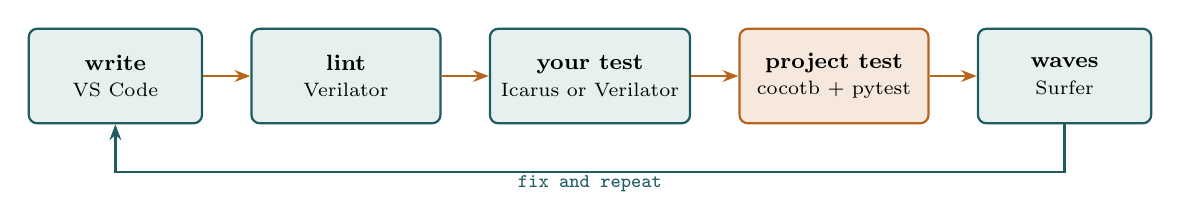
\begin{tikzpicture}[node distance=5mm and 6mm]
    \node[blk, minimum width=22mm, minimum height=12mm] (wr) {\textbf{write}\\\scriptsize VS Code};
    \node[blk, right=of wr, minimum width=24mm, minimum height=12mm] (li) {\textbf{lint}\\\scriptsize Verilator};
    \node[blk, right=of li, minimum width=24mm, minimum height=12mm] (tb) {\textbf{your test}\\\scriptsize Icarus or Verilator};
    \node[hot, right=of tb, minimum width=24mm, minimum height=12mm] (pt) {\textbf{project test}\\\scriptsize cocotb + pytest};
    \node[blk, right=of pt, minimum width=22mm, minimum height=12mm] (wv) {\textbf{waves}\\\scriptsize Surfer};
    \foreach \a/\b in {wr/li, li/tb, tb/pt, pt/wv} \draw[wire] (\a) -- (\b);
    \draw[wireb] (wv.south) -- ++(0,-6mm) -| node[lbl,pos=0.25,below]{fix and repeat} (wr.south);
  \end{tikzpicture}
  \vspace{3mm}

  \raggedright\scriptsize
\begin{lstlisting}
verilator --lint-only -Wall labs/my_rtl/pe.sv                       # lint: no output = clean
iverilog -g2012 -o pe_sim pe.sv tb_pe.sv && vvp pe_sim              # your test on Icarus
verilator --binary --timing --trace -Wno-fatal --timescale 1ns/1ps \
          --top-module tb_pe pe.sv tb_pe.sv && ./obj_dir/Vtb_pe     # the same test on Verilator
cp labs/my_rtl/pe.sv rtl/core/pe.sv && cd tb && pytest -q test_pe.py   # project test (grade)
\end{lstlisting}
\end{frame}

% =====================================================================
\begin{frame}{10.\ Common mistakes and what you will see}
  \small
  \begin{itemize}
    \item \textbf{Forgot \sig{signed}} $\rightarrow$ \sig{test\_pe.py} fails at the pair $(-128, 127)$:
          got $16\,256$, expected $-16\,256$.
    \item \textbf{\sig{clear} zeroes only \sig{acc}} $\rightarrow$ the enable-and-clear test fails on
          \sig{a\_out == 0}.
    \item \textbf{Checked \sig{en} before \sig{clear}} $\rightarrow$ a new job starts with an old total.
    \item \textbf{Used \sig{=} instead of \sig{<=}} $\rightarrow$ Verilator lint warns \sig{BLKSEQ};
          the test may still pass here, but in bigger designs it causes races.
    \item \textbf{Accumulator too narrow} (16 bits) $\rightarrow$ large random sums wrap and fail.
    \item \textbf{Product only 8 bits} $\rightarrow$ the top half of every product is lost; Verilator
          lint warns \sig{WIDTH}.
  \end{itemize}
  \vspace{2mm}
  \footnotesize\color{muted} Try each mistake on purpose (Lab 3, Part G), read the message, then undo it.
\end{frame}

% =====================================================================
\begin{frame}[fragile]{11.\ The project's PE --- look only after yours passes}
  \begin{columns}[T]
    \column{0.6\textwidth}
\begin{lstlisting}[basicstyle=\ttfamily\fontsize{6.2}{7.2}\selectfont]
module pe #(
    parameter int DW = 8,               // operand width
    parameter int AW = 32               // accumulator width
) (
    input  logic                 clk,
    input  logic                 rst_n,
    input  logic                 clear,
    input  logic                 en,
    input  logic signed [DW-1:0] a_in,
    input  logic signed [DW-1:0] b_in,
    output logic signed [DW-1:0] a_out,
    output logic signed [DW-1:0] b_out,
    output logic signed [AW-1:0] acc
);
    logic signed [2*DW-1:0] prod;
    assign prod = a_in * b_in;          // signed multiply

    always_ff @(posedge clk) begin
        if (!rst_n || clear) begin
            a_out <= '0;
            b_out <= '0;
            acc   <= '0;
        end else if (en) begin
            a_out <= a_in;
            b_out <= b_in;
            acc   <= acc + AW'(prod);    // sign-extend, add
        end
    end
endmodule
\end{lstlisting}
    \column{0.37\textwidth}\small
    \begin{itemize}
      \item \sig{prod}: the \textbf{multiplier} box, 16 bits, \sig{signed}.
      \item \sig{AW'(prod)}: the \textbf{sign-extend} box.
      \item \sig{acc + \ldots}: the \textbf{adder} box with its feedback.
      \item The three \sig{<=} lines: the three \textbf{registers}.
      \item No \sig{else} at the end: the \textbf{hold} rule.
    \end{itemize}
    \vspace{2mm}
    \footnotesize\color{muted} File: \sig{rtl/core/pe.sv}. Compare with yours using
    \sig{git diff main -- rtl/core/pe.sv}.
  \end{columns}
\end{frame}

% =====================================================================
\begin{frame}{12.\ Check yourself}
  \small
  Answer out loud, without looking back:
  \begin{enumerate}
    \item What are the three jobs of a PE every clock?
    \item Draw the inside of the PE and label every wire with its bit width.
    \item Why does \sig{clear} have to be checked before \sig{en}?
    \item Why is $(-128)\times(-128)$ \emph{not} enough to test signed multiplication?
    \item What is \sig{acc} after the MACs $(-128,-128)$, $(127,-128)$, $(5,7)$? \hfill (163)
    \item How many flip-flops are in one PE? In an 8$\times$8 array? \hfill (48; 3\,072)
    \item Why are \sig{a\_out} and \sig{b\_out} registers and not plain wires?
  \end{enumerate}
  \vspace{2mm}
  \footnotesize\color{muted} Next: Lab 4, the skew buffer --- why the inputs must arrive one cycle apart.
\end{frame}

\end{document}
